\documentclass[11pt]{amsart}
\usepackage[a4paper,margin=1in]{geometry}
\usepackage{amssymb}
\usepackage{booktabs}
\usepackage{tikz}
\usepackage[font=small,labelfont=bf]{caption}
\usepackage[hidelinks]{hyperref}

\colorlet{copper}{orange!75!black}
\definecolor{steel}{HTML}{2F5D8A}
\colorlet{inkmuted}{black!60}
\tikzset{book/thin/.style={black!55, line width=0.4pt}}

\newtheorem{theorem}{Theorem}
\newtheorem{lemma}[theorem]{Lemma}
\newtheorem{corollary}[theorem]{Corollary}
\theoremstyle{remark}
\newtheorem{remark}[theorem]{Remark}

\title{Permutations With No Whole-Number Averages}
\author{Vamshi Jandhyala}
\address{London, United Kingdom}
\email{vamshi.jandhyala@gmail.com}

\begin{document}

\begin{abstract}
Call a permutation of $1,\dots,n$ good if no block of consecutive entries, other than the whole permutation, of length at least two has an integer average. A question on MathOverflow asks whether, for odd $n$, good permutations exist exactly when $n$ is a Mersenne prime. An answer there shows that $n$ must have the form $2^m-1$. We prove that the asker's example $1,n-1,n,n-3,n-2,\dots,2,3$ is good exactly when $n=2^m-1$ is prime, and an exhaustive search shows that the composite cases $n=15$ and $n=63$ have no good permutation at all. The theorems, including the answer's, are formally verified in Lean~4.
\end{abstract}

\maketitle

\section{The question}

Take the numbers $1,\dots,7$ in the order
\[
1,\ 6,\ 7,\ 4,\ 5,\ 2,\ 3 .
\]
Pick any run of consecutive entries, of length between $2$ and $6$, and average it: $6,7$ gives $6\tfrac12$, $1,6,7$ gives $4\tfrac23$, $7,4,5,2$ gives $4\tfrac12$. None of the averages is a whole number. The whole permutation is the only exception, and it has to be: its average is $(1+\dots+7)/7=4$. Before reading on, try to do the same with $1,\dots,5$; it cannot be done.

Philip Weiss asked on MathOverflow in August 2026 \cite{MO} about such arrangements. Call a permutation $a_1,\dots,a_n$ of $1,\dots,n$ \emph{good} if every block $a_s,a_{s+1},\dots,a_e$ with $2\le e-s+1<n$ has a non-integer average. For even $n$ good permutations are easy, as Weiss noted in a comment: in $2,1,4,3,\dots,n,n-1$ every block of even length has a half-integer average, and every block of odd length $L\ge3$ has sum $\equiv\pm1\pmod L$. For odd $n$ he observed that the permutation
\begin{equation}\label{eq:c}
1,\ n-1,\ n,\ n-3,\ n-2,\ \dots,\ 2,\ 3
\end{equation}
is good when $n$ is a Mersenne prime $2^m-1$, found by search that good permutations exist for odd $n\le41$ only when $n=3,7,31$, and asked whether, for odd $n$, a good permutation exists if and only if $n$ is a Mersenne prime.

Half of the question is settled. Building on a comment by te4, Sergiu Alexandru B\^{\i}sceanu proved in an answer \cite{SAB} that $n$ must be a Mersenne number.

\begin{theorem}[B\^{\i}sceanu]\label{thm:mersenne}
If $n\ge3$ is odd and a good permutation of $1,\dots,n$ exists, then $n=2^m-1$ for some $m$.
\end{theorem}

The other half, that a composite $2^m-1$ such as $15=3\cdot5$ has no good permutation, is open. This note adds three things. Theorem~\ref{thm:asker} explains why the example~\eqref{eq:c} needs $n$ prime: its only blocks with integer average are its prefixes whose length divides $n$. The structure in B\^{\i}sceanu's proof cuts the search space by half, which takes the exhaustive search to $n=63$, the second composite Mersenne number (Theorem~\ref{thm:search}). And every theorem here, Theorem~\ref{thm:mersenne} included, is checked in Lean.

\begin{theorem}\label{thm:asker}
Let $n=2^m-1$ with $m\ge2$. A block of length $L\ge2$ in~\eqref{eq:c} has an integer average if and only if it is a prefix and $L$ divides $n$. In particular~\eqref{eq:c} is good if and only if $n$ is prime.
\end{theorem}

\begin{theorem}\label{thm:search}
For $n=7$ and $n=31$ there are exactly four good permutations: \eqref{eq:c}, its reverse, its complement $a_t\mapsto n+1-a_t$ and the reverse of the complement. For $n=15$ and $n=63$ there are none.
\end{theorem}

So the conjecture holds for every odd $n\le63$, and for $n\le31$ the good permutation is unique up to these symmetries.

\section{Why only \texorpdfstring{$2^m-1$}{2\textasciicircum m-1}}

The proof of Theorem~\ref{thm:mersenne} looks at blocks whose length is a power of two. Fix a good permutation of odd length $n\ge3$, and write $S(t,L)=a_t+\dots+a_{t+L-1}$ for the sum of the block of length $L$ starting at position $t$.

\begin{lemma}\label{lem:2adic}
If $2^k<n$ with $k\ge1$, then every block of length $2^k$ sums to an odd multiple of $2^{k-1}$. Consequently $a_{t+2^k}\equiv a_t\pmod{2^k}$ whenever both positions exist.
\end{lemma}

\begin{proof}
For $k=1$ the claim says that two neighbours have an odd sum, which is exactly the statement that their average is not an integer. Suppose the claim holds for $k$ and $2^{k+1}<n$. A block of length $2^{k+1}$ is two blocks of length $2^k$, so its sum is $2^{k-1}(o_1+o_2)$ with $o_1,o_2$ odd. That is a multiple of $2^k$. It is not a multiple of $2^{k+1}$, because the block is proper and its average is not an integer, so it is an odd multiple of $2^k$.

For the congruence, slide the block one place: $S(t+1,2^k)-S(t,2^k)=a_{t+2^k}-a_t$. Both sums are odd multiples of $2^{k-1}$, so their difference is a multiple of $2^k$.
\end{proof}

For $n=7$ the lemma says that neighbours have opposite parity, and that $a_{t+4}\equiv a_t\pmod4$. In $1,6,7,4,5,2,3$ the pairs $(a_1,a_5),(a_2,a_6),(a_3,a_7)$ are $(1,5),(6,2),(7,3)$, each differing by $4$.

\begin{proof}[Proof of Theorem~\ref{thm:mersenne}]
Let $q$ be the largest power of two below $n$ and write $n=q+s$. Since $n$ is odd and $q\ge2$ is even, $s$ is odd and $1\le s<q$. For $1\le i\le s$ the entries $a_i$ and $a_{i+q}$ are distinct numbers in $1,\dots,n$ that agree modulo $q$, by Lemma~\ref{lem:2adic}. Their difference is a nonzero multiple of $q$ and less than $2q$ in size, so it is $\pm q$: the pair is $\{x_i,x_i+q\}$ for some $x_i\le s$. Distinct $i$ give distinct $x_i$, since each value occurs once. So the $s$ pairs use up exactly the values $1,\dots,s$ and $q+1,\dots,n$, and the middle block $a_{s+1},\dots,a_q$ is a permutation of $s+1,\dots,q$. Its average is $(s+q+1)/2=(n+1)/2$, an integer. The middle block is proper, so its length $q-s$ must be $1$, and $n=2q-1$.
\end{proof}

When $n=2^m-1$ the middle block is the single entry at position $q=2^{m-1}$, and the proof gives more than the shape of $n$.

\begin{corollary}\label{cor:reduction}
If $n=2^m-1$ and $a$ is good, then $a_q=q$ for $q=2^{m-1}$, and $\{a_i,a_{i+q}\}=\{x,x+q\}$ for some $x$, for every $i<q$.
\end{corollary}

Figure~\ref{fig:pairs} shows this for $n=31$. A good permutation is determined by its first $q-1$ entries, since each later entry is the partner of the entry $q$ places earlier. That halving is what makes the search in Section~\ref{sec:search} possible.

\begin{figure}[ht]
\centering
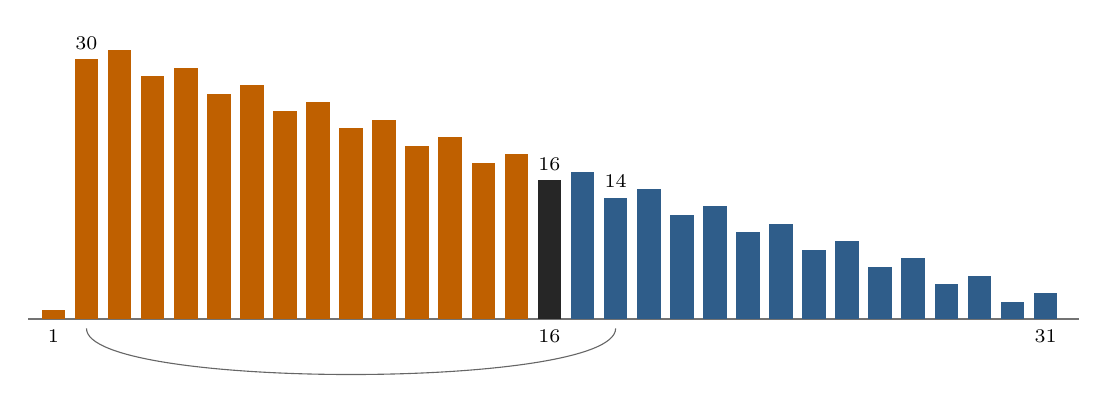
\begin{tikzpicture}
  \draw[book/thin] (0.1,0) -- (13.44,0);
\fill[copper] (0.270,0) rectangle (0.570,0.110);
\fill[copper] (0.690,0) rectangle (0.990,3.300);
\fill[copper] (1.110,0) rectangle (1.410,3.410);
\fill[copper] (1.530,0) rectangle (1.830,3.080);
\fill[copper] (1.950,0) rectangle (2.250,3.190);
\fill[copper] (2.370,0) rectangle (2.670,2.860);
\fill[copper] (2.790,0) rectangle (3.090,2.970);
\fill[copper] (3.210,0) rectangle (3.510,2.640);
\fill[copper] (3.630,0) rectangle (3.930,2.750);
\fill[copper] (4.050,0) rectangle (4.350,2.420);
\fill[copper] (4.470,0) rectangle (4.770,2.530);
\fill[copper] (4.890,0) rectangle (5.190,2.200);
\fill[copper] (5.310,0) rectangle (5.610,2.310);
\fill[copper] (5.730,0) rectangle (6.030,1.980);
\fill[copper] (6.150,0) rectangle (6.450,2.090);
\fill[black!85] (6.570,0) rectangle (6.870,1.760);
\fill[steel] (6.990,0) rectangle (7.290,1.870);
\fill[steel] (7.410,0) rectangle (7.710,1.540);
\fill[steel] (7.830,0) rectangle (8.130,1.650);
\fill[steel] (8.250,0) rectangle (8.550,1.320);
\fill[steel] (8.670,0) rectangle (8.970,1.430);
\fill[steel] (9.090,0) rectangle (9.390,1.100);
\fill[steel] (9.510,0) rectangle (9.810,1.210);
\fill[steel] (9.930,0) rectangle (10.230,0.880);
\fill[steel] (10.350,0) rectangle (10.650,0.990);
\fill[steel] (10.770,0) rectangle (11.070,0.660);
\fill[steel] (11.190,0) rectangle (11.490,0.770);
\fill[steel] (11.610,0) rectangle (11.910,0.440);
\fill[steel] (12.030,0) rectangle (12.330,0.550);
\fill[steel] (12.450,0) rectangle (12.750,0.220);
\fill[steel] (12.870,0) rectangle (13.170,0.330);
\node[above, font=\scriptsize] at (0.840,3.300) {30};
\node[above, font=\scriptsize] at (7.560,1.540) {14};
\node[above, font=\scriptsize] at (6.720,1.760) {16};
\draw[inkmuted] (0.840,-0.12) .. controls (0.840,-0.9) and (7.560,-0.9) .. (7.560,-0.12);
\node[below, font=\scriptsize] at (0.420,-0.02) {1};
\node[below, font=\scriptsize] at (6.720,-0.02) {16};
\node[below, font=\scriptsize] at (13.020,-0.02) {31};

\end{tikzpicture}
\caption{The permutation~\eqref{eq:c} for $n=31$, as bars of height $a_t$. The middle entry is $a_{16}=16$. Positions $i$ and $i+16$ hold two values $16$ apart, as Corollary~\ref{cor:reduction} requires of every good permutation; one such pair, $a_2=30$ and $a_{18}=14$, is linked.}
\label{fig:pairs}
\end{figure}

\section{The asker's permutation}

Weiss's example~\eqref{eq:c} has a closed form. Its first entry is $a_1=1$, and for $t\ge2$
\begin{equation}\label{eq:closed}
a_t=n+2-t-(-1)^t .
\end{equation}
Read the right-hand side in two parts. The line $n+2-t$ falls from $n$ at $t=2$ to $2$ at $t=n$; the term $-(-1)^t$ lowers each even position by one and raises each odd position by one, which swaps neighbours in pairs. For $n=7$ the line gives $7,6,5,4,3,2$ at $t=2,\dots,7$, and the swaps turn it into $6,7,4,5,2,3$.

\begin{proof}[Proof of Theorem~\ref{thm:asker}]
\emph{Blocks away from the start.} Take a block from position $s\ge2$ to $e$, of length $L=e-s+1\ge2$. By~\eqref{eq:closed} its average is
\[
n+2-\frac{s+e}2-\frac{\varepsilon}{L},\qquad \varepsilon=\sum_{t=s}^{e}(-1)^t\in\{-1,0,1\}.
\]
If $L$ is even, the signs cancel, $\varepsilon=0$, and $(s+e)/2$ is a half-integer. If $L$ is odd, $(s+e)/2$ is an integer and $\varepsilon=\pm1$, so the average is an integer plus $\pm1/L$ with $L\ge3$. In neither case is it an integer.

\emph{Prefixes of odd length.} Summing~\eqref{eq:closed}, the prefix of length $L=2r+1$ has sum $(2r+1)(n+1-r)-n$. Its average is an integer exactly when $L$ divides $n$.

\emph{Prefixes of even length.} The prefix of length $L=2v$ has sum $(2v-1)(n+1-v)=(2v-1)(2^m-v)$. Write $v=2^ju$ with $u$ odd. Since $v\le n<2^m$, we have $j<m$, so $2^m-v=2^j(2^{m-j}-u)$ with $2^{m-j}-u$ odd. The sum is therefore $2^j$ times an odd number, while $L=2^{j+1}u$. So $L$ does not divide the sum, and no even prefix has an integer average.

Hence the blocks with integer average are the prefixes whose length $L\ge2$ divides $n$. The prefix of length $n$ is the whole permutation and does not count, so~\eqref{eq:c} is good exactly when $n$ has no divisor $L$ with $2\le L<n$, that is, when $n$ is prime.
\end{proof}

For $n=15$ the two failures are $1+14+15=30=3\cdot10$ and $1+14+15+12+13=55=5\cdot11$, the prefixes of lengths $3$ and $5$. Figure~\ref{fig:blocks} shows every block for $n=15$ and $n=31$.

\begin{figure}[ht]
\centering
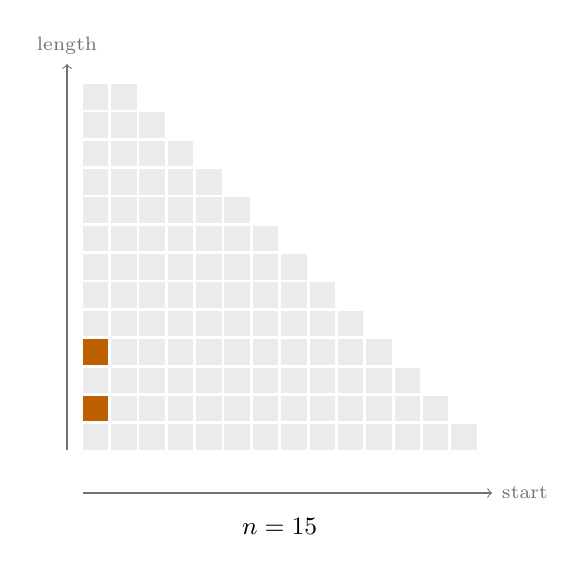
\begin{tikzpicture}
  \path[fill=black!8] (0.000,0.000) rectangle +(0.324,0.324);
\path[fill=black!8] (0.360,0.000) rectangle +(0.324,0.324);
\path[fill=black!8] (0.720,0.000) rectangle +(0.324,0.324);
\path[fill=black!8] (1.080,0.000) rectangle +(0.324,0.324);
\path[fill=black!8] (1.440,0.000) rectangle +(0.324,0.324);
\path[fill=black!8] (1.800,0.000) rectangle +(0.324,0.324);
\path[fill=black!8] (2.160,0.000) rectangle +(0.324,0.324);
\path[fill=black!8] (2.520,0.000) rectangle +(0.324,0.324);
\path[fill=black!8] (2.880,0.000) rectangle +(0.324,0.324);
\path[fill=black!8] (3.240,0.000) rectangle +(0.324,0.324);
\path[fill=black!8] (3.600,0.000) rectangle +(0.324,0.324);
\path[fill=black!8] (3.960,0.000) rectangle +(0.324,0.324);
\path[fill=black!8] (4.320,0.000) rectangle +(0.324,0.324);
\path[fill=black!8] (4.680,0.000) rectangle +(0.324,0.324);
\path[fill=copper] (0.000,0.360) rectangle +(0.324,0.324);
\path[fill=black!8] (0.360,0.360) rectangle +(0.324,0.324);
\path[fill=black!8] (0.720,0.360) rectangle +(0.324,0.324);
\path[fill=black!8] (1.080,0.360) rectangle +(0.324,0.324);
\path[fill=black!8] (1.440,0.360) rectangle +(0.324,0.324);
\path[fill=black!8] (1.800,0.360) rectangle +(0.324,0.324);
\path[fill=black!8] (2.160,0.360) rectangle +(0.324,0.324);
\path[fill=black!8] (2.520,0.360) rectangle +(0.324,0.324);
\path[fill=black!8] (2.880,0.360) rectangle +(0.324,0.324);
\path[fill=black!8] (3.240,0.360) rectangle +(0.324,0.324);
\path[fill=black!8] (3.600,0.360) rectangle +(0.324,0.324);
\path[fill=black!8] (3.960,0.360) rectangle +(0.324,0.324);
\path[fill=black!8] (4.320,0.360) rectangle +(0.324,0.324);
\path[fill=black!8] (0.000,0.720) rectangle +(0.324,0.324);
\path[fill=black!8] (0.360,0.720) rectangle +(0.324,0.324);
\path[fill=black!8] (0.720,0.720) rectangle +(0.324,0.324);
\path[fill=black!8] (1.080,0.720) rectangle +(0.324,0.324);
\path[fill=black!8] (1.440,0.720) rectangle +(0.324,0.324);
\path[fill=black!8] (1.800,0.720) rectangle +(0.324,0.324);
\path[fill=black!8] (2.160,0.720) rectangle +(0.324,0.324);
\path[fill=black!8] (2.520,0.720) rectangle +(0.324,0.324);
\path[fill=black!8] (2.880,0.720) rectangle +(0.324,0.324);
\path[fill=black!8] (3.240,0.720) rectangle +(0.324,0.324);
\path[fill=black!8] (3.600,0.720) rectangle +(0.324,0.324);
\path[fill=black!8] (3.960,0.720) rectangle +(0.324,0.324);
\path[fill=copper] (0.000,1.080) rectangle +(0.324,0.324);
\path[fill=black!8] (0.360,1.080) rectangle +(0.324,0.324);
\path[fill=black!8] (0.720,1.080) rectangle +(0.324,0.324);
\path[fill=black!8] (1.080,1.080) rectangle +(0.324,0.324);
\path[fill=black!8] (1.440,1.080) rectangle +(0.324,0.324);
\path[fill=black!8] (1.800,1.080) rectangle +(0.324,0.324);
\path[fill=black!8] (2.160,1.080) rectangle +(0.324,0.324);
\path[fill=black!8] (2.520,1.080) rectangle +(0.324,0.324);
\path[fill=black!8] (2.880,1.080) rectangle +(0.324,0.324);
\path[fill=black!8] (3.240,1.080) rectangle +(0.324,0.324);
\path[fill=black!8] (3.600,1.080) rectangle +(0.324,0.324);
\path[fill=black!8] (0.000,1.440) rectangle +(0.324,0.324);
\path[fill=black!8] (0.360,1.440) rectangle +(0.324,0.324);
\path[fill=black!8] (0.720,1.440) rectangle +(0.324,0.324);
\path[fill=black!8] (1.080,1.440) rectangle +(0.324,0.324);
\path[fill=black!8] (1.440,1.440) rectangle +(0.324,0.324);
\path[fill=black!8] (1.800,1.440) rectangle +(0.324,0.324);
\path[fill=black!8] (2.160,1.440) rectangle +(0.324,0.324);
\path[fill=black!8] (2.520,1.440) rectangle +(0.324,0.324);
\path[fill=black!8] (2.880,1.440) rectangle +(0.324,0.324);
\path[fill=black!8] (3.240,1.440) rectangle +(0.324,0.324);
\path[fill=black!8] (0.000,1.800) rectangle +(0.324,0.324);
\path[fill=black!8] (0.360,1.800) rectangle +(0.324,0.324);
\path[fill=black!8] (0.720,1.800) rectangle +(0.324,0.324);
\path[fill=black!8] (1.080,1.800) rectangle +(0.324,0.324);
\path[fill=black!8] (1.440,1.800) rectangle +(0.324,0.324);
\path[fill=black!8] (1.800,1.800) rectangle +(0.324,0.324);
\path[fill=black!8] (2.160,1.800) rectangle +(0.324,0.324);
\path[fill=black!8] (2.520,1.800) rectangle +(0.324,0.324);
\path[fill=black!8] (2.880,1.800) rectangle +(0.324,0.324);
\path[fill=black!8] (0.000,2.160) rectangle +(0.324,0.324);
\path[fill=black!8] (0.360,2.160) rectangle +(0.324,0.324);
\path[fill=black!8] (0.720,2.160) rectangle +(0.324,0.324);
\path[fill=black!8] (1.080,2.160) rectangle +(0.324,0.324);
\path[fill=black!8] (1.440,2.160) rectangle +(0.324,0.324);
\path[fill=black!8] (1.800,2.160) rectangle +(0.324,0.324);
\path[fill=black!8] (2.160,2.160) rectangle +(0.324,0.324);
\path[fill=black!8] (2.520,2.160) rectangle +(0.324,0.324);
\path[fill=black!8] (0.000,2.520) rectangle +(0.324,0.324);
\path[fill=black!8] (0.360,2.520) rectangle +(0.324,0.324);
\path[fill=black!8] (0.720,2.520) rectangle +(0.324,0.324);
\path[fill=black!8] (1.080,2.520) rectangle +(0.324,0.324);
\path[fill=black!8] (1.440,2.520) rectangle +(0.324,0.324);
\path[fill=black!8] (1.800,2.520) rectangle +(0.324,0.324);
\path[fill=black!8] (2.160,2.520) rectangle +(0.324,0.324);
\path[fill=black!8] (0.000,2.880) rectangle +(0.324,0.324);
\path[fill=black!8] (0.360,2.880) rectangle +(0.324,0.324);
\path[fill=black!8] (0.720,2.880) rectangle +(0.324,0.324);
\path[fill=black!8] (1.080,2.880) rectangle +(0.324,0.324);
\path[fill=black!8] (1.440,2.880) rectangle +(0.324,0.324);
\path[fill=black!8] (1.800,2.880) rectangle +(0.324,0.324);
\path[fill=black!8] (0.000,3.240) rectangle +(0.324,0.324);
\path[fill=black!8] (0.360,3.240) rectangle +(0.324,0.324);
\path[fill=black!8] (0.720,3.240) rectangle +(0.324,0.324);
\path[fill=black!8] (1.080,3.240) rectangle +(0.324,0.324);
\path[fill=black!8] (1.440,3.240) rectangle +(0.324,0.324);
\path[fill=black!8] (0.000,3.600) rectangle +(0.324,0.324);
\path[fill=black!8] (0.360,3.600) rectangle +(0.324,0.324);
\path[fill=black!8] (0.720,3.600) rectangle +(0.324,0.324);
\path[fill=black!8] (1.080,3.600) rectangle +(0.324,0.324);
\path[fill=black!8] (0.000,3.960) rectangle +(0.324,0.324);
\path[fill=black!8] (0.360,3.960) rectangle +(0.324,0.324);
\path[fill=black!8] (0.720,3.960) rectangle +(0.324,0.324);
\path[fill=black!8] (0.000,4.320) rectangle +(0.324,0.324);
\path[fill=black!8] (0.360,4.320) rectangle +(0.324,0.324);

  \node[below, font=\small] at (2.5,-0.75) {$n=15$};
  \draw[->, book/thin] (-0.2,0) -- (-0.2,4.9) node[above, font=\scriptsize] {length};
  \draw[->, book/thin] (0,-0.55) -- (5.2,-0.55) node[right, font=\scriptsize] {start};
\end{tikzpicture}\qquad
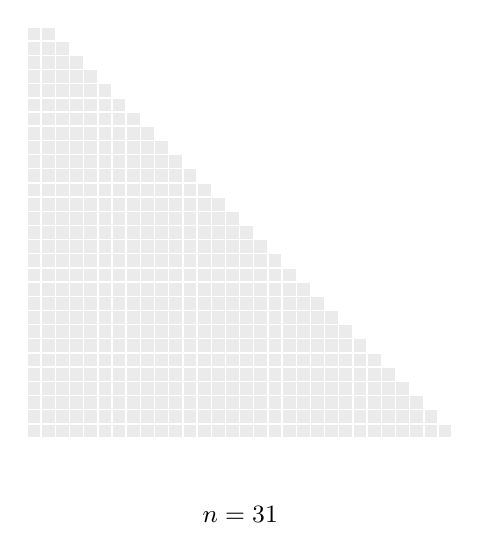
\begin{tikzpicture}
  \path[fill=black!8] (0.000,0.000) rectangle +(0.162,0.162);
\path[fill=black!8] (0.180,0.000) rectangle +(0.162,0.162);
\path[fill=black!8] (0.360,0.000) rectangle +(0.162,0.162);
\path[fill=black!8] (0.540,0.000) rectangle +(0.162,0.162);
\path[fill=black!8] (0.720,0.000) rectangle +(0.162,0.162);
\path[fill=black!8] (0.900,0.000) rectangle +(0.162,0.162);
\path[fill=black!8] (1.080,0.000) rectangle +(0.162,0.162);
\path[fill=black!8] (1.260,0.000) rectangle +(0.162,0.162);
\path[fill=black!8] (1.440,0.000) rectangle +(0.162,0.162);
\path[fill=black!8] (1.620,0.000) rectangle +(0.162,0.162);
\path[fill=black!8] (1.800,0.000) rectangle +(0.162,0.162);
\path[fill=black!8] (1.980,0.000) rectangle +(0.162,0.162);
\path[fill=black!8] (2.160,0.000) rectangle +(0.162,0.162);
\path[fill=black!8] (2.340,0.000) rectangle +(0.162,0.162);
\path[fill=black!8] (2.520,0.000) rectangle +(0.162,0.162);
\path[fill=black!8] (2.700,0.000) rectangle +(0.162,0.162);
\path[fill=black!8] (2.880,0.000) rectangle +(0.162,0.162);
\path[fill=black!8] (3.060,0.000) rectangle +(0.162,0.162);
\path[fill=black!8] (3.240,0.000) rectangle +(0.162,0.162);
\path[fill=black!8] (3.420,0.000) rectangle +(0.162,0.162);
\path[fill=black!8] (3.600,0.000) rectangle +(0.162,0.162);
\path[fill=black!8] (3.780,0.000) rectangle +(0.162,0.162);
\path[fill=black!8] (3.960,0.000) rectangle +(0.162,0.162);
\path[fill=black!8] (4.140,0.000) rectangle +(0.162,0.162);
\path[fill=black!8] (4.320,0.000) rectangle +(0.162,0.162);
\path[fill=black!8] (4.500,0.000) rectangle +(0.162,0.162);
\path[fill=black!8] (4.680,0.000) rectangle +(0.162,0.162);
\path[fill=black!8] (4.860,0.000) rectangle +(0.162,0.162);
\path[fill=black!8] (5.040,0.000) rectangle +(0.162,0.162);
\path[fill=black!8] (5.220,0.000) rectangle +(0.162,0.162);
\path[fill=black!8] (0.000,0.180) rectangle +(0.162,0.162);
\path[fill=black!8] (0.180,0.180) rectangle +(0.162,0.162);
\path[fill=black!8] (0.360,0.180) rectangle +(0.162,0.162);
\path[fill=black!8] (0.540,0.180) rectangle +(0.162,0.162);
\path[fill=black!8] (0.720,0.180) rectangle +(0.162,0.162);
\path[fill=black!8] (0.900,0.180) rectangle +(0.162,0.162);
\path[fill=black!8] (1.080,0.180) rectangle +(0.162,0.162);
\path[fill=black!8] (1.260,0.180) rectangle +(0.162,0.162);
\path[fill=black!8] (1.440,0.180) rectangle +(0.162,0.162);
\path[fill=black!8] (1.620,0.180) rectangle +(0.162,0.162);
\path[fill=black!8] (1.800,0.180) rectangle +(0.162,0.162);
\path[fill=black!8] (1.980,0.180) rectangle +(0.162,0.162);
\path[fill=black!8] (2.160,0.180) rectangle +(0.162,0.162);
\path[fill=black!8] (2.340,0.180) rectangle +(0.162,0.162);
\path[fill=black!8] (2.520,0.180) rectangle +(0.162,0.162);
\path[fill=black!8] (2.700,0.180) rectangle +(0.162,0.162);
\path[fill=black!8] (2.880,0.180) rectangle +(0.162,0.162);
\path[fill=black!8] (3.060,0.180) rectangle +(0.162,0.162);
\path[fill=black!8] (3.240,0.180) rectangle +(0.162,0.162);
\path[fill=black!8] (3.420,0.180) rectangle +(0.162,0.162);
\path[fill=black!8] (3.600,0.180) rectangle +(0.162,0.162);
\path[fill=black!8] (3.780,0.180) rectangle +(0.162,0.162);
\path[fill=black!8] (3.960,0.180) rectangle +(0.162,0.162);
\path[fill=black!8] (4.140,0.180) rectangle +(0.162,0.162);
\path[fill=black!8] (4.320,0.180) rectangle +(0.162,0.162);
\path[fill=black!8] (4.500,0.180) rectangle +(0.162,0.162);
\path[fill=black!8] (4.680,0.180) rectangle +(0.162,0.162);
\path[fill=black!8] (4.860,0.180) rectangle +(0.162,0.162);
\path[fill=black!8] (5.040,0.180) rectangle +(0.162,0.162);
\path[fill=black!8] (0.000,0.360) rectangle +(0.162,0.162);
\path[fill=black!8] (0.180,0.360) rectangle +(0.162,0.162);
\path[fill=black!8] (0.360,0.360) rectangle +(0.162,0.162);
\path[fill=black!8] (0.540,0.360) rectangle +(0.162,0.162);
\path[fill=black!8] (0.720,0.360) rectangle +(0.162,0.162);
\path[fill=black!8] (0.900,0.360) rectangle +(0.162,0.162);
\path[fill=black!8] (1.080,0.360) rectangle +(0.162,0.162);
\path[fill=black!8] (1.260,0.360) rectangle +(0.162,0.162);
\path[fill=black!8] (1.440,0.360) rectangle +(0.162,0.162);
\path[fill=black!8] (1.620,0.360) rectangle +(0.162,0.162);
\path[fill=black!8] (1.800,0.360) rectangle +(0.162,0.162);
\path[fill=black!8] (1.980,0.360) rectangle +(0.162,0.162);
\path[fill=black!8] (2.160,0.360) rectangle +(0.162,0.162);
\path[fill=black!8] (2.340,0.360) rectangle +(0.162,0.162);
\path[fill=black!8] (2.520,0.360) rectangle +(0.162,0.162);
\path[fill=black!8] (2.700,0.360) rectangle +(0.162,0.162);
\path[fill=black!8] (2.880,0.360) rectangle +(0.162,0.162);
\path[fill=black!8] (3.060,0.360) rectangle +(0.162,0.162);
\path[fill=black!8] (3.240,0.360) rectangle +(0.162,0.162);
\path[fill=black!8] (3.420,0.360) rectangle +(0.162,0.162);
\path[fill=black!8] (3.600,0.360) rectangle +(0.162,0.162);
\path[fill=black!8] (3.780,0.360) rectangle +(0.162,0.162);
\path[fill=black!8] (3.960,0.360) rectangle +(0.162,0.162);
\path[fill=black!8] (4.140,0.360) rectangle +(0.162,0.162);
\path[fill=black!8] (4.320,0.360) rectangle +(0.162,0.162);
\path[fill=black!8] (4.500,0.360) rectangle +(0.162,0.162);
\path[fill=black!8] (4.680,0.360) rectangle +(0.162,0.162);
\path[fill=black!8] (4.860,0.360) rectangle +(0.162,0.162);
\path[fill=black!8] (0.000,0.540) rectangle +(0.162,0.162);
\path[fill=black!8] (0.180,0.540) rectangle +(0.162,0.162);
\path[fill=black!8] (0.360,0.540) rectangle +(0.162,0.162);
\path[fill=black!8] (0.540,0.540) rectangle +(0.162,0.162);
\path[fill=black!8] (0.720,0.540) rectangle +(0.162,0.162);
\path[fill=black!8] (0.900,0.540) rectangle +(0.162,0.162);
\path[fill=black!8] (1.080,0.540) rectangle +(0.162,0.162);
\path[fill=black!8] (1.260,0.540) rectangle +(0.162,0.162);
\path[fill=black!8] (1.440,0.540) rectangle +(0.162,0.162);
\path[fill=black!8] (1.620,0.540) rectangle +(0.162,0.162);
\path[fill=black!8] (1.800,0.540) rectangle +(0.162,0.162);
\path[fill=black!8] (1.980,0.540) rectangle +(0.162,0.162);
\path[fill=black!8] (2.160,0.540) rectangle +(0.162,0.162);
\path[fill=black!8] (2.340,0.540) rectangle +(0.162,0.162);
\path[fill=black!8] (2.520,0.540) rectangle +(0.162,0.162);
\path[fill=black!8] (2.700,0.540) rectangle +(0.162,0.162);
\path[fill=black!8] (2.880,0.540) rectangle +(0.162,0.162);
\path[fill=black!8] (3.060,0.540) rectangle +(0.162,0.162);
\path[fill=black!8] (3.240,0.540) rectangle +(0.162,0.162);
\path[fill=black!8] (3.420,0.540) rectangle +(0.162,0.162);
\path[fill=black!8] (3.600,0.540) rectangle +(0.162,0.162);
\path[fill=black!8] (3.780,0.540) rectangle +(0.162,0.162);
\path[fill=black!8] (3.960,0.540) rectangle +(0.162,0.162);
\path[fill=black!8] (4.140,0.540) rectangle +(0.162,0.162);
\path[fill=black!8] (4.320,0.540) rectangle +(0.162,0.162);
\path[fill=black!8] (4.500,0.540) rectangle +(0.162,0.162);
\path[fill=black!8] (4.680,0.540) rectangle +(0.162,0.162);
\path[fill=black!8] (0.000,0.720) rectangle +(0.162,0.162);
\path[fill=black!8] (0.180,0.720) rectangle +(0.162,0.162);
\path[fill=black!8] (0.360,0.720) rectangle +(0.162,0.162);
\path[fill=black!8] (0.540,0.720) rectangle +(0.162,0.162);
\path[fill=black!8] (0.720,0.720) rectangle +(0.162,0.162);
\path[fill=black!8] (0.900,0.720) rectangle +(0.162,0.162);
\path[fill=black!8] (1.080,0.720) rectangle +(0.162,0.162);
\path[fill=black!8] (1.260,0.720) rectangle +(0.162,0.162);
\path[fill=black!8] (1.440,0.720) rectangle +(0.162,0.162);
\path[fill=black!8] (1.620,0.720) rectangle +(0.162,0.162);
\path[fill=black!8] (1.800,0.720) rectangle +(0.162,0.162);
\path[fill=black!8] (1.980,0.720) rectangle +(0.162,0.162);
\path[fill=black!8] (2.160,0.720) rectangle +(0.162,0.162);
\path[fill=black!8] (2.340,0.720) rectangle +(0.162,0.162);
\path[fill=black!8] (2.520,0.720) rectangle +(0.162,0.162);
\path[fill=black!8] (2.700,0.720) rectangle +(0.162,0.162);
\path[fill=black!8] (2.880,0.720) rectangle +(0.162,0.162);
\path[fill=black!8] (3.060,0.720) rectangle +(0.162,0.162);
\path[fill=black!8] (3.240,0.720) rectangle +(0.162,0.162);
\path[fill=black!8] (3.420,0.720) rectangle +(0.162,0.162);
\path[fill=black!8] (3.600,0.720) rectangle +(0.162,0.162);
\path[fill=black!8] (3.780,0.720) rectangle +(0.162,0.162);
\path[fill=black!8] (3.960,0.720) rectangle +(0.162,0.162);
\path[fill=black!8] (4.140,0.720) rectangle +(0.162,0.162);
\path[fill=black!8] (4.320,0.720) rectangle +(0.162,0.162);
\path[fill=black!8] (4.500,0.720) rectangle +(0.162,0.162);
\path[fill=black!8] (0.000,0.900) rectangle +(0.162,0.162);
\path[fill=black!8] (0.180,0.900) rectangle +(0.162,0.162);
\path[fill=black!8] (0.360,0.900) rectangle +(0.162,0.162);
\path[fill=black!8] (0.540,0.900) rectangle +(0.162,0.162);
\path[fill=black!8] (0.720,0.900) rectangle +(0.162,0.162);
\path[fill=black!8] (0.900,0.900) rectangle +(0.162,0.162);
\path[fill=black!8] (1.080,0.900) rectangle +(0.162,0.162);
\path[fill=black!8] (1.260,0.900) rectangle +(0.162,0.162);
\path[fill=black!8] (1.440,0.900) rectangle +(0.162,0.162);
\path[fill=black!8] (1.620,0.900) rectangle +(0.162,0.162);
\path[fill=black!8] (1.800,0.900) rectangle +(0.162,0.162);
\path[fill=black!8] (1.980,0.900) rectangle +(0.162,0.162);
\path[fill=black!8] (2.160,0.900) rectangle +(0.162,0.162);
\path[fill=black!8] (2.340,0.900) rectangle +(0.162,0.162);
\path[fill=black!8] (2.520,0.900) rectangle +(0.162,0.162);
\path[fill=black!8] (2.700,0.900) rectangle +(0.162,0.162);
\path[fill=black!8] (2.880,0.900) rectangle +(0.162,0.162);
\path[fill=black!8] (3.060,0.900) rectangle +(0.162,0.162);
\path[fill=black!8] (3.240,0.900) rectangle +(0.162,0.162);
\path[fill=black!8] (3.420,0.900) rectangle +(0.162,0.162);
\path[fill=black!8] (3.600,0.900) rectangle +(0.162,0.162);
\path[fill=black!8] (3.780,0.900) rectangle +(0.162,0.162);
\path[fill=black!8] (3.960,0.900) rectangle +(0.162,0.162);
\path[fill=black!8] (4.140,0.900) rectangle +(0.162,0.162);
\path[fill=black!8] (4.320,0.900) rectangle +(0.162,0.162);
\path[fill=black!8] (0.000,1.080) rectangle +(0.162,0.162);
\path[fill=black!8] (0.180,1.080) rectangle +(0.162,0.162);
\path[fill=black!8] (0.360,1.080) rectangle +(0.162,0.162);
\path[fill=black!8] (0.540,1.080) rectangle +(0.162,0.162);
\path[fill=black!8] (0.720,1.080) rectangle +(0.162,0.162);
\path[fill=black!8] (0.900,1.080) rectangle +(0.162,0.162);
\path[fill=black!8] (1.080,1.080) rectangle +(0.162,0.162);
\path[fill=black!8] (1.260,1.080) rectangle +(0.162,0.162);
\path[fill=black!8] (1.440,1.080) rectangle +(0.162,0.162);
\path[fill=black!8] (1.620,1.080) rectangle +(0.162,0.162);
\path[fill=black!8] (1.800,1.080) rectangle +(0.162,0.162);
\path[fill=black!8] (1.980,1.080) rectangle +(0.162,0.162);
\path[fill=black!8] (2.160,1.080) rectangle +(0.162,0.162);
\path[fill=black!8] (2.340,1.080) rectangle +(0.162,0.162);
\path[fill=black!8] (2.520,1.080) rectangle +(0.162,0.162);
\path[fill=black!8] (2.700,1.080) rectangle +(0.162,0.162);
\path[fill=black!8] (2.880,1.080) rectangle +(0.162,0.162);
\path[fill=black!8] (3.060,1.080) rectangle +(0.162,0.162);
\path[fill=black!8] (3.240,1.080) rectangle +(0.162,0.162);
\path[fill=black!8] (3.420,1.080) rectangle +(0.162,0.162);
\path[fill=black!8] (3.600,1.080) rectangle +(0.162,0.162);
\path[fill=black!8] (3.780,1.080) rectangle +(0.162,0.162);
\path[fill=black!8] (3.960,1.080) rectangle +(0.162,0.162);
\path[fill=black!8] (4.140,1.080) rectangle +(0.162,0.162);
\path[fill=black!8] (0.000,1.260) rectangle +(0.162,0.162);
\path[fill=black!8] (0.180,1.260) rectangle +(0.162,0.162);
\path[fill=black!8] (0.360,1.260) rectangle +(0.162,0.162);
\path[fill=black!8] (0.540,1.260) rectangle +(0.162,0.162);
\path[fill=black!8] (0.720,1.260) rectangle +(0.162,0.162);
\path[fill=black!8] (0.900,1.260) rectangle +(0.162,0.162);
\path[fill=black!8] (1.080,1.260) rectangle +(0.162,0.162);
\path[fill=black!8] (1.260,1.260) rectangle +(0.162,0.162);
\path[fill=black!8] (1.440,1.260) rectangle +(0.162,0.162);
\path[fill=black!8] (1.620,1.260) rectangle +(0.162,0.162);
\path[fill=black!8] (1.800,1.260) rectangle +(0.162,0.162);
\path[fill=black!8] (1.980,1.260) rectangle +(0.162,0.162);
\path[fill=black!8] (2.160,1.260) rectangle +(0.162,0.162);
\path[fill=black!8] (2.340,1.260) rectangle +(0.162,0.162);
\path[fill=black!8] (2.520,1.260) rectangle +(0.162,0.162);
\path[fill=black!8] (2.700,1.260) rectangle +(0.162,0.162);
\path[fill=black!8] (2.880,1.260) rectangle +(0.162,0.162);
\path[fill=black!8] (3.060,1.260) rectangle +(0.162,0.162);
\path[fill=black!8] (3.240,1.260) rectangle +(0.162,0.162);
\path[fill=black!8] (3.420,1.260) rectangle +(0.162,0.162);
\path[fill=black!8] (3.600,1.260) rectangle +(0.162,0.162);
\path[fill=black!8] (3.780,1.260) rectangle +(0.162,0.162);
\path[fill=black!8] (3.960,1.260) rectangle +(0.162,0.162);
\path[fill=black!8] (0.000,1.440) rectangle +(0.162,0.162);
\path[fill=black!8] (0.180,1.440) rectangle +(0.162,0.162);
\path[fill=black!8] (0.360,1.440) rectangle +(0.162,0.162);
\path[fill=black!8] (0.540,1.440) rectangle +(0.162,0.162);
\path[fill=black!8] (0.720,1.440) rectangle +(0.162,0.162);
\path[fill=black!8] (0.900,1.440) rectangle +(0.162,0.162);
\path[fill=black!8] (1.080,1.440) rectangle +(0.162,0.162);
\path[fill=black!8] (1.260,1.440) rectangle +(0.162,0.162);
\path[fill=black!8] (1.440,1.440) rectangle +(0.162,0.162);
\path[fill=black!8] (1.620,1.440) rectangle +(0.162,0.162);
\path[fill=black!8] (1.800,1.440) rectangle +(0.162,0.162);
\path[fill=black!8] (1.980,1.440) rectangle +(0.162,0.162);
\path[fill=black!8] (2.160,1.440) rectangle +(0.162,0.162);
\path[fill=black!8] (2.340,1.440) rectangle +(0.162,0.162);
\path[fill=black!8] (2.520,1.440) rectangle +(0.162,0.162);
\path[fill=black!8] (2.700,1.440) rectangle +(0.162,0.162);
\path[fill=black!8] (2.880,1.440) rectangle +(0.162,0.162);
\path[fill=black!8] (3.060,1.440) rectangle +(0.162,0.162);
\path[fill=black!8] (3.240,1.440) rectangle +(0.162,0.162);
\path[fill=black!8] (3.420,1.440) rectangle +(0.162,0.162);
\path[fill=black!8] (3.600,1.440) rectangle +(0.162,0.162);
\path[fill=black!8] (3.780,1.440) rectangle +(0.162,0.162);
\path[fill=black!8] (0.000,1.620) rectangle +(0.162,0.162);
\path[fill=black!8] (0.180,1.620) rectangle +(0.162,0.162);
\path[fill=black!8] (0.360,1.620) rectangle +(0.162,0.162);
\path[fill=black!8] (0.540,1.620) rectangle +(0.162,0.162);
\path[fill=black!8] (0.720,1.620) rectangle +(0.162,0.162);
\path[fill=black!8] (0.900,1.620) rectangle +(0.162,0.162);
\path[fill=black!8] (1.080,1.620) rectangle +(0.162,0.162);
\path[fill=black!8] (1.260,1.620) rectangle +(0.162,0.162);
\path[fill=black!8] (1.440,1.620) rectangle +(0.162,0.162);
\path[fill=black!8] (1.620,1.620) rectangle +(0.162,0.162);
\path[fill=black!8] (1.800,1.620) rectangle +(0.162,0.162);
\path[fill=black!8] (1.980,1.620) rectangle +(0.162,0.162);
\path[fill=black!8] (2.160,1.620) rectangle +(0.162,0.162);
\path[fill=black!8] (2.340,1.620) rectangle +(0.162,0.162);
\path[fill=black!8] (2.520,1.620) rectangle +(0.162,0.162);
\path[fill=black!8] (2.700,1.620) rectangle +(0.162,0.162);
\path[fill=black!8] (2.880,1.620) rectangle +(0.162,0.162);
\path[fill=black!8] (3.060,1.620) rectangle +(0.162,0.162);
\path[fill=black!8] (3.240,1.620) rectangle +(0.162,0.162);
\path[fill=black!8] (3.420,1.620) rectangle +(0.162,0.162);
\path[fill=black!8] (3.600,1.620) rectangle +(0.162,0.162);
\path[fill=black!8] (0.000,1.800) rectangle +(0.162,0.162);
\path[fill=black!8] (0.180,1.800) rectangle +(0.162,0.162);
\path[fill=black!8] (0.360,1.800) rectangle +(0.162,0.162);
\path[fill=black!8] (0.540,1.800) rectangle +(0.162,0.162);
\path[fill=black!8] (0.720,1.800) rectangle +(0.162,0.162);
\path[fill=black!8] (0.900,1.800) rectangle +(0.162,0.162);
\path[fill=black!8] (1.080,1.800) rectangle +(0.162,0.162);
\path[fill=black!8] (1.260,1.800) rectangle +(0.162,0.162);
\path[fill=black!8] (1.440,1.800) rectangle +(0.162,0.162);
\path[fill=black!8] (1.620,1.800) rectangle +(0.162,0.162);
\path[fill=black!8] (1.800,1.800) rectangle +(0.162,0.162);
\path[fill=black!8] (1.980,1.800) rectangle +(0.162,0.162);
\path[fill=black!8] (2.160,1.800) rectangle +(0.162,0.162);
\path[fill=black!8] (2.340,1.800) rectangle +(0.162,0.162);
\path[fill=black!8] (2.520,1.800) rectangle +(0.162,0.162);
\path[fill=black!8] (2.700,1.800) rectangle +(0.162,0.162);
\path[fill=black!8] (2.880,1.800) rectangle +(0.162,0.162);
\path[fill=black!8] (3.060,1.800) rectangle +(0.162,0.162);
\path[fill=black!8] (3.240,1.800) rectangle +(0.162,0.162);
\path[fill=black!8] (3.420,1.800) rectangle +(0.162,0.162);
\path[fill=black!8] (0.000,1.980) rectangle +(0.162,0.162);
\path[fill=black!8] (0.180,1.980) rectangle +(0.162,0.162);
\path[fill=black!8] (0.360,1.980) rectangle +(0.162,0.162);
\path[fill=black!8] (0.540,1.980) rectangle +(0.162,0.162);
\path[fill=black!8] (0.720,1.980) rectangle +(0.162,0.162);
\path[fill=black!8] (0.900,1.980) rectangle +(0.162,0.162);
\path[fill=black!8] (1.080,1.980) rectangle +(0.162,0.162);
\path[fill=black!8] (1.260,1.980) rectangle +(0.162,0.162);
\path[fill=black!8] (1.440,1.980) rectangle +(0.162,0.162);
\path[fill=black!8] (1.620,1.980) rectangle +(0.162,0.162);
\path[fill=black!8] (1.800,1.980) rectangle +(0.162,0.162);
\path[fill=black!8] (1.980,1.980) rectangle +(0.162,0.162);
\path[fill=black!8] (2.160,1.980) rectangle +(0.162,0.162);
\path[fill=black!8] (2.340,1.980) rectangle +(0.162,0.162);
\path[fill=black!8] (2.520,1.980) rectangle +(0.162,0.162);
\path[fill=black!8] (2.700,1.980) rectangle +(0.162,0.162);
\path[fill=black!8] (2.880,1.980) rectangle +(0.162,0.162);
\path[fill=black!8] (3.060,1.980) rectangle +(0.162,0.162);
\path[fill=black!8] (3.240,1.980) rectangle +(0.162,0.162);
\path[fill=black!8] (0.000,2.160) rectangle +(0.162,0.162);
\path[fill=black!8] (0.180,2.160) rectangle +(0.162,0.162);
\path[fill=black!8] (0.360,2.160) rectangle +(0.162,0.162);
\path[fill=black!8] (0.540,2.160) rectangle +(0.162,0.162);
\path[fill=black!8] (0.720,2.160) rectangle +(0.162,0.162);
\path[fill=black!8] (0.900,2.160) rectangle +(0.162,0.162);
\path[fill=black!8] (1.080,2.160) rectangle +(0.162,0.162);
\path[fill=black!8] (1.260,2.160) rectangle +(0.162,0.162);
\path[fill=black!8] (1.440,2.160) rectangle +(0.162,0.162);
\path[fill=black!8] (1.620,2.160) rectangle +(0.162,0.162);
\path[fill=black!8] (1.800,2.160) rectangle +(0.162,0.162);
\path[fill=black!8] (1.980,2.160) rectangle +(0.162,0.162);
\path[fill=black!8] (2.160,2.160) rectangle +(0.162,0.162);
\path[fill=black!8] (2.340,2.160) rectangle +(0.162,0.162);
\path[fill=black!8] (2.520,2.160) rectangle +(0.162,0.162);
\path[fill=black!8] (2.700,2.160) rectangle +(0.162,0.162);
\path[fill=black!8] (2.880,2.160) rectangle +(0.162,0.162);
\path[fill=black!8] (3.060,2.160) rectangle +(0.162,0.162);
\path[fill=black!8] (0.000,2.340) rectangle +(0.162,0.162);
\path[fill=black!8] (0.180,2.340) rectangle +(0.162,0.162);
\path[fill=black!8] (0.360,2.340) rectangle +(0.162,0.162);
\path[fill=black!8] (0.540,2.340) rectangle +(0.162,0.162);
\path[fill=black!8] (0.720,2.340) rectangle +(0.162,0.162);
\path[fill=black!8] (0.900,2.340) rectangle +(0.162,0.162);
\path[fill=black!8] (1.080,2.340) rectangle +(0.162,0.162);
\path[fill=black!8] (1.260,2.340) rectangle +(0.162,0.162);
\path[fill=black!8] (1.440,2.340) rectangle +(0.162,0.162);
\path[fill=black!8] (1.620,2.340) rectangle +(0.162,0.162);
\path[fill=black!8] (1.800,2.340) rectangle +(0.162,0.162);
\path[fill=black!8] (1.980,2.340) rectangle +(0.162,0.162);
\path[fill=black!8] (2.160,2.340) rectangle +(0.162,0.162);
\path[fill=black!8] (2.340,2.340) rectangle +(0.162,0.162);
\path[fill=black!8] (2.520,2.340) rectangle +(0.162,0.162);
\path[fill=black!8] (2.700,2.340) rectangle +(0.162,0.162);
\path[fill=black!8] (2.880,2.340) rectangle +(0.162,0.162);
\path[fill=black!8] (0.000,2.520) rectangle +(0.162,0.162);
\path[fill=black!8] (0.180,2.520) rectangle +(0.162,0.162);
\path[fill=black!8] (0.360,2.520) rectangle +(0.162,0.162);
\path[fill=black!8] (0.540,2.520) rectangle +(0.162,0.162);
\path[fill=black!8] (0.720,2.520) rectangle +(0.162,0.162);
\path[fill=black!8] (0.900,2.520) rectangle +(0.162,0.162);
\path[fill=black!8] (1.080,2.520) rectangle +(0.162,0.162);
\path[fill=black!8] (1.260,2.520) rectangle +(0.162,0.162);
\path[fill=black!8] (1.440,2.520) rectangle +(0.162,0.162);
\path[fill=black!8] (1.620,2.520) rectangle +(0.162,0.162);
\path[fill=black!8] (1.800,2.520) rectangle +(0.162,0.162);
\path[fill=black!8] (1.980,2.520) rectangle +(0.162,0.162);
\path[fill=black!8] (2.160,2.520) rectangle +(0.162,0.162);
\path[fill=black!8] (2.340,2.520) rectangle +(0.162,0.162);
\path[fill=black!8] (2.520,2.520) rectangle +(0.162,0.162);
\path[fill=black!8] (2.700,2.520) rectangle +(0.162,0.162);
\path[fill=black!8] (0.000,2.700) rectangle +(0.162,0.162);
\path[fill=black!8] (0.180,2.700) rectangle +(0.162,0.162);
\path[fill=black!8] (0.360,2.700) rectangle +(0.162,0.162);
\path[fill=black!8] (0.540,2.700) rectangle +(0.162,0.162);
\path[fill=black!8] (0.720,2.700) rectangle +(0.162,0.162);
\path[fill=black!8] (0.900,2.700) rectangle +(0.162,0.162);
\path[fill=black!8] (1.080,2.700) rectangle +(0.162,0.162);
\path[fill=black!8] (1.260,2.700) rectangle +(0.162,0.162);
\path[fill=black!8] (1.440,2.700) rectangle +(0.162,0.162);
\path[fill=black!8] (1.620,2.700) rectangle +(0.162,0.162);
\path[fill=black!8] (1.800,2.700) rectangle +(0.162,0.162);
\path[fill=black!8] (1.980,2.700) rectangle +(0.162,0.162);
\path[fill=black!8] (2.160,2.700) rectangle +(0.162,0.162);
\path[fill=black!8] (2.340,2.700) rectangle +(0.162,0.162);
\path[fill=black!8] (2.520,2.700) rectangle +(0.162,0.162);
\path[fill=black!8] (0.000,2.880) rectangle +(0.162,0.162);
\path[fill=black!8] (0.180,2.880) rectangle +(0.162,0.162);
\path[fill=black!8] (0.360,2.880) rectangle +(0.162,0.162);
\path[fill=black!8] (0.540,2.880) rectangle +(0.162,0.162);
\path[fill=black!8] (0.720,2.880) rectangle +(0.162,0.162);
\path[fill=black!8] (0.900,2.880) rectangle +(0.162,0.162);
\path[fill=black!8] (1.080,2.880) rectangle +(0.162,0.162);
\path[fill=black!8] (1.260,2.880) rectangle +(0.162,0.162);
\path[fill=black!8] (1.440,2.880) rectangle +(0.162,0.162);
\path[fill=black!8] (1.620,2.880) rectangle +(0.162,0.162);
\path[fill=black!8] (1.800,2.880) rectangle +(0.162,0.162);
\path[fill=black!8] (1.980,2.880) rectangle +(0.162,0.162);
\path[fill=black!8] (2.160,2.880) rectangle +(0.162,0.162);
\path[fill=black!8] (2.340,2.880) rectangle +(0.162,0.162);
\path[fill=black!8] (0.000,3.060) rectangle +(0.162,0.162);
\path[fill=black!8] (0.180,3.060) rectangle +(0.162,0.162);
\path[fill=black!8] (0.360,3.060) rectangle +(0.162,0.162);
\path[fill=black!8] (0.540,3.060) rectangle +(0.162,0.162);
\path[fill=black!8] (0.720,3.060) rectangle +(0.162,0.162);
\path[fill=black!8] (0.900,3.060) rectangle +(0.162,0.162);
\path[fill=black!8] (1.080,3.060) rectangle +(0.162,0.162);
\path[fill=black!8] (1.260,3.060) rectangle +(0.162,0.162);
\path[fill=black!8] (1.440,3.060) rectangle +(0.162,0.162);
\path[fill=black!8] (1.620,3.060) rectangle +(0.162,0.162);
\path[fill=black!8] (1.800,3.060) rectangle +(0.162,0.162);
\path[fill=black!8] (1.980,3.060) rectangle +(0.162,0.162);
\path[fill=black!8] (2.160,3.060) rectangle +(0.162,0.162);
\path[fill=black!8] (0.000,3.240) rectangle +(0.162,0.162);
\path[fill=black!8] (0.180,3.240) rectangle +(0.162,0.162);
\path[fill=black!8] (0.360,3.240) rectangle +(0.162,0.162);
\path[fill=black!8] (0.540,3.240) rectangle +(0.162,0.162);
\path[fill=black!8] (0.720,3.240) rectangle +(0.162,0.162);
\path[fill=black!8] (0.900,3.240) rectangle +(0.162,0.162);
\path[fill=black!8] (1.080,3.240) rectangle +(0.162,0.162);
\path[fill=black!8] (1.260,3.240) rectangle +(0.162,0.162);
\path[fill=black!8] (1.440,3.240) rectangle +(0.162,0.162);
\path[fill=black!8] (1.620,3.240) rectangle +(0.162,0.162);
\path[fill=black!8] (1.800,3.240) rectangle +(0.162,0.162);
\path[fill=black!8] (1.980,3.240) rectangle +(0.162,0.162);
\path[fill=black!8] (0.000,3.420) rectangle +(0.162,0.162);
\path[fill=black!8] (0.180,3.420) rectangle +(0.162,0.162);
\path[fill=black!8] (0.360,3.420) rectangle +(0.162,0.162);
\path[fill=black!8] (0.540,3.420) rectangle +(0.162,0.162);
\path[fill=black!8] (0.720,3.420) rectangle +(0.162,0.162);
\path[fill=black!8] (0.900,3.420) rectangle +(0.162,0.162);
\path[fill=black!8] (1.080,3.420) rectangle +(0.162,0.162);
\path[fill=black!8] (1.260,3.420) rectangle +(0.162,0.162);
\path[fill=black!8] (1.440,3.420) rectangle +(0.162,0.162);
\path[fill=black!8] (1.620,3.420) rectangle +(0.162,0.162);
\path[fill=black!8] (1.800,3.420) rectangle +(0.162,0.162);
\path[fill=black!8] (0.000,3.600) rectangle +(0.162,0.162);
\path[fill=black!8] (0.180,3.600) rectangle +(0.162,0.162);
\path[fill=black!8] (0.360,3.600) rectangle +(0.162,0.162);
\path[fill=black!8] (0.540,3.600) rectangle +(0.162,0.162);
\path[fill=black!8] (0.720,3.600) rectangle +(0.162,0.162);
\path[fill=black!8] (0.900,3.600) rectangle +(0.162,0.162);
\path[fill=black!8] (1.080,3.600) rectangle +(0.162,0.162);
\path[fill=black!8] (1.260,3.600) rectangle +(0.162,0.162);
\path[fill=black!8] (1.440,3.600) rectangle +(0.162,0.162);
\path[fill=black!8] (1.620,3.600) rectangle +(0.162,0.162);
\path[fill=black!8] (0.000,3.780) rectangle +(0.162,0.162);
\path[fill=black!8] (0.180,3.780) rectangle +(0.162,0.162);
\path[fill=black!8] (0.360,3.780) rectangle +(0.162,0.162);
\path[fill=black!8] (0.540,3.780) rectangle +(0.162,0.162);
\path[fill=black!8] (0.720,3.780) rectangle +(0.162,0.162);
\path[fill=black!8] (0.900,3.780) rectangle +(0.162,0.162);
\path[fill=black!8] (1.080,3.780) rectangle +(0.162,0.162);
\path[fill=black!8] (1.260,3.780) rectangle +(0.162,0.162);
\path[fill=black!8] (1.440,3.780) rectangle +(0.162,0.162);
\path[fill=black!8] (0.000,3.960) rectangle +(0.162,0.162);
\path[fill=black!8] (0.180,3.960) rectangle +(0.162,0.162);
\path[fill=black!8] (0.360,3.960) rectangle +(0.162,0.162);
\path[fill=black!8] (0.540,3.960) rectangle +(0.162,0.162);
\path[fill=black!8] (0.720,3.960) rectangle +(0.162,0.162);
\path[fill=black!8] (0.900,3.960) rectangle +(0.162,0.162);
\path[fill=black!8] (1.080,3.960) rectangle +(0.162,0.162);
\path[fill=black!8] (1.260,3.960) rectangle +(0.162,0.162);
\path[fill=black!8] (0.000,4.140) rectangle +(0.162,0.162);
\path[fill=black!8] (0.180,4.140) rectangle +(0.162,0.162);
\path[fill=black!8] (0.360,4.140) rectangle +(0.162,0.162);
\path[fill=black!8] (0.540,4.140) rectangle +(0.162,0.162);
\path[fill=black!8] (0.720,4.140) rectangle +(0.162,0.162);
\path[fill=black!8] (0.900,4.140) rectangle +(0.162,0.162);
\path[fill=black!8] (1.080,4.140) rectangle +(0.162,0.162);
\path[fill=black!8] (0.000,4.320) rectangle +(0.162,0.162);
\path[fill=black!8] (0.180,4.320) rectangle +(0.162,0.162);
\path[fill=black!8] (0.360,4.320) rectangle +(0.162,0.162);
\path[fill=black!8] (0.540,4.320) rectangle +(0.162,0.162);
\path[fill=black!8] (0.720,4.320) rectangle +(0.162,0.162);
\path[fill=black!8] (0.900,4.320) rectangle +(0.162,0.162);
\path[fill=black!8] (0.000,4.500) rectangle +(0.162,0.162);
\path[fill=black!8] (0.180,4.500) rectangle +(0.162,0.162);
\path[fill=black!8] (0.360,4.500) rectangle +(0.162,0.162);
\path[fill=black!8] (0.540,4.500) rectangle +(0.162,0.162);
\path[fill=black!8] (0.720,4.500) rectangle +(0.162,0.162);
\path[fill=black!8] (0.000,4.680) rectangle +(0.162,0.162);
\path[fill=black!8] (0.180,4.680) rectangle +(0.162,0.162);
\path[fill=black!8] (0.360,4.680) rectangle +(0.162,0.162);
\path[fill=black!8] (0.540,4.680) rectangle +(0.162,0.162);
\path[fill=black!8] (0.000,4.860) rectangle +(0.162,0.162);
\path[fill=black!8] (0.180,4.860) rectangle +(0.162,0.162);
\path[fill=black!8] (0.360,4.860) rectangle +(0.162,0.162);
\path[fill=black!8] (0.000,5.040) rectangle +(0.162,0.162);
\path[fill=black!8] (0.180,5.040) rectangle +(0.162,0.162);

  \node[below, font=\small] at (2.7,-0.75) {$n=31$};
\end{tikzpicture}
\caption{Every proper block of~\eqref{eq:c} of length at least $2$: the cell in column $s$ and row $L$ is the block of length $L$ starting at position $s$. Filled cells have an integer average. For $n=15$ they are the prefixes of lengths $3$ and $5$, the proper divisors of $15$; for the prime $n=31$ there are none.}
\label{fig:blocks}
\end{figure}

\section{Searching the composite cases}\label{sec:search}

For $n=2^m-1$, Corollary~\ref{cor:reduction} reduces the search to choosing $a_1,\dots,a_{q-1}$. Choosing $a_t$ also fixes $a_{t+q}$, so when $a_t$ is placed one can test every block inside positions $1,\dots,t$ and every block inside positions $q+1,\dots,q+t$ at once. A depth-first search with these tests, followed by a full check of each completed permutation, gives the counts in Table~\ref{tab:counts}.

\begin{table}[ht]
\centering
\begin{tabular}{rrrr}
\toprule
$n$ & good permutations & search nodes & plain search \\
\midrule
$7$ & $4$ & $23$ & $4$ \\
$15$ & $0$ & $855$ & $0$ \\
$31$ & $4$ & $85{,}387$ & $4$ \\
$63$ & $0$ & $106{,}605{,}579$ & -- \\
\bottomrule
\end{tabular}
\caption{Exhaustive counts for $n=2^m-1$ with the reduction of Corollary~\ref{cor:reduction}, and with a plain search that uses no structure.}
\label{tab:counts}
\end{table}

A second program, a plain depth-first search with no structural assumption, confirms the counts for $n=7,15,31$ and finds no good permutation for any other odd $n\le41$, which reproduces Weiss's search. It cannot reach $n=63$. Its running time grows by a factor of about $2.5$ with each step of $n$ by two, so $n=63$ would take about a month.

\begin{remark}
For $n=15$ the obstruction lies in the block lengths $3$ and $5$ that divide $n$, as it does for~\eqref{eq:c}. If the conditions for those two lengths are dropped and every other length is kept, the reduced search finds $320$ permutations. A proof for composite $2^m-1$ would have to use the divisors of $n$, which the powers of two in Lemma~\ref{lem:2adic} do not see.
\end{remark}

The next composite Mersenne number after $63$ is $255$, far beyond this search; the next prime case, $n=127$, would take hours and would test whether the good permutation stays unique up to symmetry.

\section{Verification}

Theorem~\ref{thm:mersenne} (with Lemma~\ref{lem:2adic}), Corollary~\ref{cor:reduction} and Theorem~\ref{thm:asker}, including the fact that~\eqref{eq:c} is a permutation, are proved in Lean~4 with Mathlib~\cite{mathlib}, using only the standard axioms; ten planted errors in the statements and definitions all fail to compile. The searches of Theorem~\ref{thm:search} are two C programs driven by a Python script, which also checks Theorem~\ref{thm:asker} directly for $n\le2047$; the reduced search runs only on the structure that Lean proves, and a planted error in it (skipping the lengths that divide $n$) is caught. Code and Lean files are at~\cite{repo}.

\section*{Acknowledgments}

The question and the permutation~\eqref{eq:c} are Philip Weiss's; the $2$-adic congruence is from a comment by te4, and Theorem~\ref{thm:mersenne} is Sergiu Alexandru B\^{\i}sceanu's. Peter Taylor reported partial searches in a comment. The proof of Theorem~\ref{thm:asker}, the searches and the Lean formalisation were carried out with Claude Opus~5.5 (Anthropic). The author is responsible for the content.

\begin{thebibliography}{9}
\bibitem{MO} P.~Weiss, \emph{Do only Mersenne primes have ``good'' permutations?}, MathOverflow question 514690 (2026), \url{https://mathoverflow.net/q/514690}.
\bibitem{SAB} S.~A.~B\^{\i}sceanu, answer to~\cite{MO}, MathOverflow answer 514702 (2026), \url{https://mathoverflow.net/a/514702}.
\bibitem{mathlib} The mathlib Community, \emph{The Lean mathematical library}, in: Proc. 9th ACM SIGPLAN Int. Conf. on Certified Programs and Proofs (CPP 2020), 367--381.
\bibitem{repo} V.~Jandhyala, code and Lean proofs, \url{https://github.com/jvvk/mathematics/tree/main/good-permutations-mersenne}.
\end{thebibliography}

\end{document}
